\documentclass[10pt]{article}
\usepackage[%
left=0.984252in,%
right=0.787402in,%
top=0.787402in,%
bottom=0.787402in,%
paperheight=11in,%
paperwidth=8.5in%
]{geometry}%

\usepackage{xeCJK}
\usepackage{blindtext}
\usepackage[T1]{fontenc}
\usepackage{caption}
\usepackage{graphicx}
\usepackage{textcomp}
\usepackage{fancyhdr}

\pagestyle{fancy}
\fancyhf{}
\fancyhead[R]{\thepage}
\usepackage{float}
\usepackage{alltt}

\setCJKmainfont{AozoraMinchoRegular.ttf}
\setCJKsansfont{AozoraMincho-bold.ttf}


\setCJKmainfont{AozoraMinchoRegular.ttf}
\setCJKsansfont{AozoraMincho-bold.ttf}

\usepackage{indentfirst}

\title{ネットワーク実験レポート}
\author{18NC021 \thanks{情報通信基礎実験1}}
\date{カトリ スザン}
\captionsetup[table]{name=表}
\captionsetup[figure]{name=図}

\begin{document}

\begin{titlepage}
	\maketitle
    \begin{center}
        天気(1週目) 曇り, 25度, 64\% \\
        天気(2週目) 曇り, 25度, 60\% 
    \end{center}
    
\end{titlepage}

\tableofcontents
\pagebreak

\section{目的}
LANを構築することにより、LANで用いられるケーブルや機器などの構成要素と機能を理解する。インターネットで使用される TCP/IP プロトコルについて、LANで用いられるプロトコルの概要を理解する。\\ また、PCのコマンドなどを用いて、ネットワークの動作状態の確認やトラブルシューティングの方法を理解する。

\section{実験1 LANケーブルの作成}

\subsection{実施事項}
\begin{itemize}
    \item ストレートケーブルの作成
\end{itemize}
LANケーブルを作る作業を体験し、UTPケーブル内の4ペアのツイストの状態とRJ45プラグを観察することでレイヤ1の仕様の概略を理解する。

\subsection{使用機器類と構成}
CAT5eケーブル、RJ45プラグ、プラグブーツ、ニッパー、ストリッパー、圧着工具、ケーブルテスタ 

\subsection{実施手順}
この実験の中でPCをスイッチに接続するために用いるストレートケーブルを作成する。図1のようにT568Bの仕様のピン結線で、CAT5eケーブルの両端にRJ45プラグを取り付ける。プラグのピンに対して誤った配線をするとプラグを切り捨てて再度作り直しとなるので、圧着する前に十分に確認すること。\\ ケーブル先端の撚りをとる長さは、プラグの中で13mm程度である。ケーブルのスリーブはプラグの中に収まり、プラグのストッパーの爪により押さえられることを確認する。 出来上がったケーブルは、ケーブルテスタで導通とワイヤのペアが正しいことを確認する。ペアが異なると直流では通電するが、LANケーブルとしては正常に動作しない。

\section{実験2 Switchを使用したLANの構築}

\subsection{実施事項}
\begin{itemize}
    \item ケーブルと機器の接続 
    \item IPアドレスの設定
    \item ネットワークの動作状態の確認
\end{itemize}

小規模なLANを構築するときの装置構成、IPアドレスの設計と設定方法を理解する。また、ネットワークの動作状態の確認方法を理解する。

\subsection{使用機器類と構成}
switch、PC4台、作成したストレートケーブル 
\begin{figure}[H]
		\centering
		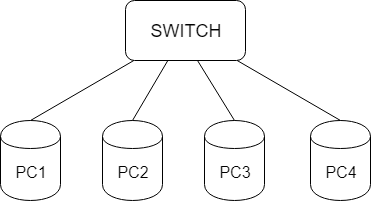
\includegraphics[width=0.5\textwidth]{networkExpreriment.png}
		\caption{実験1回路図}
	\end{figure}

\subsection{実施手順}
\begin{enumerate}
    \item ケーブルと機器の接続 \\
            図1のように、switchにストレートケーブルを用いてPCと接続する。switchのリンクインジケータが点灯していることを確認する。 
    \item \\
        IPを用いて通信を行うときには、PCなどのホストにIPアドレスを付与する必要がある。IPアドレスは手作業で固定的に設定する方法と動的に割り当てて設定する方法がある。現在ではDHCPで自動的に設定することが多いが、実験ではIPアドレスを手作業で設定する。
        \begin{itemize}
            \item ホストアドレスとサブネットマスクを各PCに割り当てる。
                実験ではクラスCネットワークのLANを作るので、次の1つのネットワークアドレスを用いる。 ネットワークアドレス 192.168.x.0 サブネットマスク 255.255.255.0 PCのホストアドレス 192.168.x.1 からホスト部に増加して各PCに付与 \\ \text{*}ここで、第3オクテッドのxは、実験グループごとに割り当てる番号とする。
            \item PCのホストアドレスとサブネットマスクを表1に記入する。
            \item IPアドレスとサブネットマスクをPCに設定する。
        \end{itemize}
        画面左下の[スタートボタン]を右クリックし、[ネットワーク接続]を選択する。\\  次に、[ローカルエリア接続※注]のデバイスを右クリックし、[プロパティ]を選択する。\\  \text{*}注:[ローカルエリア接続]は、PCによっては[イーサネット]や[Ethernet]などで表示される。\\  [インターネットプロトコルバージョン4(TCP/IPv4)]をクリックして選択し、[プロパティ]をクリックする。\\  [次のIPアドレスを使う]にチェックして、IPアドレスの情報を入力する。\\  設定の後に、[OK]をクリックして各ウィンドウを閉じる。 \\
    \item 設定したIPアドレス情報とMACアドレスの確認
            コマンドプロンプトからコマンドを入力して、設定されたIPアドレス情報とMACアドレスを確認する。
            \begin{itemize}
                \item スタートボタン]を右クリックし、[コマンドプロンプト]を選択してコマンドプロンプトを起動する。
                \item promptコマンドを入力し、プロンプトの表示を時間とPC名に変更する。  プロンプトを表示させてからコマンドを入力すると、時間が表示されるので記録が整理しやすい。
                     \\\\
                    C:\textbackslash Windows> prompt \$T\$SPC18\$G\$S \\
                    20:12:11.51 PC18>
                    \\
                \item コマンドプロンプトから次のコマンドを入力し、設定されたIPアドレス情報とMACアドレスを確認する。表示されたMACアドレスを表1に記入する。
                \\\\
                C:\textbackslash>ipconfig /all
                \\\\
                表示例  物理アドレス・・・・:00-16-26-F6-1C-30 \\
                IPv4アドレス・・・・:192.168.1.1 \\
                サブネットマスク・・・・:255.255.255.0 \\
                    
            \end{itemize}
            \begingroup
            \setlength{\tabcolsep}{5pt} % Default value: 6pt
            \renewcommand{\arraystretch}{1.5} % Default value: 1
            \begin{table}[H]
            \centering
        	\caption{各PCのアドレス情報の値}
        	\begin{tabular}{|l|l|l|l|}
        	    \hline
        	    PC & MACアドレス & IPアドレス (ホスト) & サブネットマスク\\[0.5ex]
        		\hline\hline
        	PC1 & B0-99-28-D8-11-88 & 192.168.1.2 & 255.255.255.0 \\ \hline
            PC2 & E4-7F-B2-11-C3-B8 & 192.168.1.3 & 255.255.255.0 \\ \hline
            PC3 & E4-7F-B2-11-C3-77 & 192.168.1.4 & 255.255.255.0 \\ \hline
            PC4 & B0-99-28-D8-11-71 & 192.168.1.5 & 255.255.255.0 \\ \hline
        	\end{tabular}
        \end{table} 
        \endgroup
        
    \item ネットワークの動作状態の確認
    PCコマンドなどを用いてネットワークの動作確認を行い、その結果を理解する。 リンクインジケータ(LED)の点灯を確認することで、レイヤ1の物理的な接続を確認できる。 PCからpingコマンドを実行することで、ICMPによるレイヤ3のIPアドレスによる接続の清浄性を確認できる。 
    \begin{itemize}
        \item 各PCについて、LANへの接続状態を確認して表2に記入する。
        \item pingコマンドをループバックアドレスの127.0.0.1に対して実行し、PCのTCP/IPプロトコルが正常に動作していることを確認する。その結果を表3に記入する。
        
        \begingroup
            \setlength{\tabcolsep}{5pt} % Default value: 6pt
            \renewcommand{\arraystretch}{1.5} % Default value: 1
            \begin{table}[H]
            \centering
        	\caption{各PCについての接続状態の確認結果}
        	\begin{tabular}{|c|c|c|}
        	    \hline
        	    PC &  switch/PCのリンクインジケータ  & ループバックへのping結果\\
        	    & (LED)の点灯有無 & \\ [0.5ex] 
        		\hline\hline
                	PC1 & 有 & < 1ms\\ \hline
                    PC2 & 有 & < 1ms\\ \hline
                    PC3 & 有 & < 1ms\\ \hline
                    PC4 & 有 & < 1ms\\ \hline
        	\end{tabular}
        \end{table} 
        \endgroup
        
        \item 他のPCに対するping結果の確認について、表3に記入する。
        \begingroup
            \setlength{\tabcolsep}{5pt} % Default value: 6pt
            \renewcommand{\arraystretch}{1.5} % Default value: 1
            \begin{table}[H]
            \centering
        	\caption{他のPCへの接続性の確認結果}
        	\begin{tabular}{|c|c|c|c|c|c|}
        	    \hline
        	    \multicolumn{2}{|c}{下は操作するPC} & \multicolumn{1}{|c|}{PC1} & \multicolumn{1}{|c|}{PC2} & \multicolumn{1}{|c|}{PC3} & \multicolumn{1}{|c|}{PC4}\\ \hline
        	     
        		\hline\hline
        	        PC1 & ping & < 1ms & < 1ms & < 1ms & < 1ms \\ 
        	        & HTTP & 成功 & 成功 & 成功 & 成功 \\ \hline
        	        PC2 & ping & < 1ms & < 1ms & < 1ms & < 1ms \\ 
        	        & HTTP & 成功 & 成功 & 成功 & 成功 \\ \hline
        	        PC3 & ping & < 1ms & < 1ms & < 1ms & < 1ms \\ 
        	        & HTTP & 成功 & 成功 & 成功 & 成功 \\ \hline
        	        PC4 & ping & < 1ms & < 1ms & < 1ms & < 1ms \\ 
        	        & HTTP & 成功 & 成功 & 成功 & 成功 \\ \hline
            
        	\end{tabular}
        \end{table} 
        \endgroup
        ブラウザを用いたHTTPによる接続の確認により、アプリケーション層まで正常に動作していることが確認できる。
        
        \item ブラウザで他のPCにIPアドレスを指定してアクセスする。HTTPアクセスの成否を確認し、結果を表3のHTTPの欄に記入する。 \\ なお、ブラウザは受け取った情報をキャッシュしてしまい、古い情報や状態を表示し続けることが多いので、F5を押下するかブラウザを再起動するなどして最新の状態を表示させる。
        \item 各 PCでHTTPサーバが起動していない場合は、スタートメニューかデスクトップのアイコンから、HTTPサーバソフトウェアのApacheを起動する。ディスプレイの右下のApacheのアイコンを右クリックし、さらに右クリックをして[Start]を選択してApacheを起動する。
    \end{itemize}
\end{enumerate}

\pagebreak

\section{実験3 撚りを解いたケーブルでの通信}

\subsection{実施事項}

\begin{itemize}
    \item 撚りを解いたケーブルでの通信状態を観察する。
\end{itemize}
撚りを解いたケーブルの不安定な通信状態とLANの規格に対して通信可能な距離が短いなどの通信に与える影響を観察して、ツイストペアケーブルの撚りの効果を確認する。

\subsection{使用機器類と構成}
PC(PC19)、撚りを解いたケーブル(3m, 5m)、100mストレートケーブル\\
ケーブル延長アダプタ(ストレートアダプタ、クロスアダプタ)\\ リンクインジケータ(LED)のないPCの場合は、PC間にSwitchを入れて観察する。
\begin{figure}[H]
		\centering
		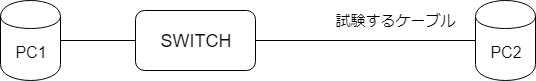
\includegraphics[width=0.7\textwidth]{zuni.png}
		\caption{実験1回路図}
	\end{figure}

\subsection{実施手順}

\begin{enumerate}
    \item IPアドレスの設定の確認 \\
    2台のPCに設定されたIPアドレスとサブネットマスクを確認する。設定については、4.2を参照のこと。
    \item 撚りを解いたケーブルでの通信状態の観察
    \begin{itemize}
        \item PC同士を試験するケーブルで接続し、リンクインジケータやpingの結果を用いて通信状態を観察する。
    \end{itemize}
    
    測定結果を表4に記入し、ケーブルの長さと通信の可否などを確認する。結果がケーブルの位置などの状態やPCの個体差により変化するので、複数回試みて不安定な状況や点灯するインジケータの表示の仕方の違いなどを観察して記録する。\\正常なツイストペアケーブルの通信可能な距離を100BASE-TXの規格を調べて比較する。
    
\end{enumerate}

\begingroup
        \setlength{\tabcolsep}{5pt} % Default value: 6pt
        \renewcommand{\arraystretch}{1.5} % Default value: 1
        \begin{table}[H]
        \centering
    	\caption{撚りを解いたケーブルでの通信状態の観察結果}
    	\begin{tabular}{|c|c|c|c|}
    	    \hline
    	    ケーブル長 &  リンクインジケーター  & ping動作結果 & ping応答がある時の\\
    	    & の点灯有無 & & 最大時間\\ [0.5ex] 
    		\hline\hline
    			3m & 時々点灯 & 失敗 & - \\ \hline
    			5m & 時々点灯 & 失敗 & -\\ \hline
    			10m & 時々点灯 & 失敗 & -\\ \hline
            	100mツイスト & 有 & 成功 & < 1ms\\ \hline
                
    	\end{tabular}
    \end{table} 
\endgroup

\pagebreak

\section{実験4 パケットのモニタリング}

\subsection{実施事項}

\begin{itemize}
    \item 実験4  パケットのモニタリング ・実施事項  
    \item ARPとICMPの動作確認
\end{itemize}
パケットキャプチャソフトを用いてパケットをモニタすることで、フレームとパケットのフォーマットの仕様を確認する。また、フレームとパケットの動きをモニタしてTCP/IP通信のプロトコルの概略を理解する。

\subsection{使用機器と構成}
パケットキャプチャソフト、Switch、PC4台

\subsection{実施手順}
ここでは、Ethernetで実行されるARPの動作とpingコマンドによるICMPの動作を確認する。また、時間に余裕があれば、HTTPの動作も確認するとよい。

\begin{enumerate}
    \item IPアドレスの設定の確認 \\
        PCに設定されたIPアドレスとサブネットマスクを確認する。設定については、4.2を参照。
    \item モニタリングの準備
        windowsのプロトコルがTCP/IPの実験のモニタリングの邪魔をしないようにwindowsのプロトコルの動作を止めておく。
    \begin{itemize}
        \item 左下の[スタートボタン]を右クリックし、[ネットワーク接続]を選択する。\\
            次に、[ローカルエリア接続]のデバイスを右クリックし、[プロパティ]をクリックする。[インターネットプロトコルバージョン4(TCP/IPv4)]以外のチェックを外す。前出の図10を参照のこと。なお、通信する他のプログラムを停止しておくと、ARPとICMPのトラヒックだけのトラヒックを得やすくなる。\\  実施結果のデータは実験グループで共有すればよいが、各自のオリジナルの実験結果を得る場合は、次のARPテーブルのクリアから③のモニタリングまでを、PC1※のところを各自が担当するPCごとに人数分(PCごとに)繰り返して実施すればよい。
        \item RPテーブルをクリアする。全PCで行う。\\\\
            C:>arp -d * \\
        \item RPテーブルの内容を表示する。この時点でMACアドレスの記憶はされていない。\\\\
        c:>arp -a \\
        ARPエントリが見つかりませんでした。 
    \end{itemize}
    
    \item  モニタリング
        \begin{itemize}
            \item キャプチャを開始する。操作は7.3を参照のこと
            \item PC1から他の1台のPC※にpingコマンドを実行する。\\
            これにより、ICMPのパケットが出されるが、それを先行してARPが行われる。\\\\
                C:>ping 192.168.4.2  \text{*}PC1以外のPCに対して行う \\
        
        
            \item ARPテーブルを表示し、表5に記入する。\\  表示された相手のPCのMACアドレスの値が表2の値に等しいことを確認する。\\\\
                     C:>arp -a \\
                        ARPテーブルの表示例  
                        インターフェース: 192.168.x.1 ̶-0xe \\ 
                        インターネット アドレス  物理アドレス  種類\\   
                        192.168.x.2 \hspace{1cm} 00-1b-8b-79-84-02\hspace{0.3cm}   動的 \\\\
             \text{*}第1オクテッドの値が、224以上のマルチキャストアドレスが表示される場合は、実験ではこれらを無視して取り扱う。
             \pagebreak
             \item キャプチャを停止する。\\
             ARPとICMPのトラヒックがキャプチャできたら、キャプチャを停止する。
         \end{itemize}
    \item ARPとICMPの動作の確認 \\
        ARPテーブルの表示からARPテーブルの情報の内容を確認し、キャプチャした結果からフレームとパケットの存在を確認して表5に記入する。
        
        \begingroup
        \setlength{\tabcolsep}{5pt} % Default value: 6pt
        \renewcommand{\arraystretch}{1.5} % Default value: 1
        \begin{table}[H]
        \centering
    	\caption{存在を確認する項目の確認結果}
    	\begin{tabular}{|c|c|c|c|} 
    	\hline
    	    存在を確認する項目 & pingしたPC & pingされたPC & それ以外のPC \\
    	    \hline\hline
    	    ARPテーブルのMACア &  192.168.1.3  & 192.168.1.2 & 192.168.1.4\\
    	    ドレスとIPアドレスの値 & E4-7F-B2-11-C3-B8 & B0-99-28-d8-11-88 & 192.168.1.5\\ [0.5ex] 
    		\hline
    			ARP request フレーム & 有 & 有 & 有 \\ \hline
    			ARP reply フレーム & 有 & 有 & 無 \\ \hline
    			ICMP Echo request & 有 & 有 & 無 \\ \hline
            	ICMP Echo reply & 有 & 有 & 無 \\ \hline
                
            	\end{tabular}
            \end{table} 
        \endgroup
        \text{*}ARPテーブルの情報はARPコマンドの結果から記入し、その他は存在する有無を記入する\\\\
        キャプチャした結果からARPフレームのEthernetヘッダの内容を分析する。
        \begin{itemize}
            \item 最初のフレームになるARP request のフレームの内容を表6に記入する。\\
            ARPフレームの宛先のMACアドレスがブロードキャストアドレスになっている。ping先のIPアドレスが入っている。また、送信元のIPアドレスとMACアドレも入っているのでそれに対して返信をすることができる。
            
                \begingroup
                \setlength{\tabcolsep}{5pt} % Default value: 6pt
                \renewcommand{\arraystretch}{1.5} % Default value: 1
                \begin{table}[H]
                \centering
            	\caption{ARP request のフレーム}
            	\begin{tabular}{|c|c|c|} 
                	\hline
                	    送信元MACアドレス &  宛先MACアドレス  & Ethernet II、Source:送信元\\
                	     B0-99-28-D8-11-88 &  ff-ff-ff-ff-ff-ff & Destination:宛先\\ [0.5ex] 
                	\hline
                	    送信元IPアドレス &  問合せのIPアドレス  & ARPデータのSender IP、\\
                	     192.168.1.2 & 192.168.1.3  & Target IP\\ [0.5ex] 
                	\hline
                \end{tabular}
                \end{table} 
                \endgroup
                \text{*}※MACアドレスは16進数で記入する\\
            
            \item ARP requestの応答であるARP replyのフレームの内容を表7に記入する。\\
            ARP replyにはping先のPCのMACアドレスが入っている。また、送信元のMACアドレスと宛先のMACアドレスが入れ替わっている。
                \begingroup
                    \setlength{\tabcolsep}{5pt} % Default value: 6pt
                    \renewcommand{\arraystretch}{1.5} % Default value: 1
                    \begin{table}[H]
                    \centering
                	\caption{ARP reply のフレーム}
                	\begin{tabular}{|c|c|c|} 
                    	\hline
                    	    送信元MACアドレス &  宛先MACアドレス  & Ethernet II、Source:送信元\\
                    	    E4-7F-B2-11-C3-B8  & B0-99-28-D8-11-88 & Destination:宛先\\ [0.5ex] 
                    	\hline
                    	    送信元IPアドレス &  問合せのIPアドレス  & ARPデータのSender IP、\\
                    	     192.168.1.3 & 192.168.1.2  & Target IP\\ [0.5ex] 
                    	\hline
                    \end{tabular}
                    \end{table} 
                    \endgroup
            \item pingコマンドが送信するICMPのEcho requestパケットを分析し、表8に記入する。ICMPではレイヤ3のIPパケットの存在とIPパケットの構造を確認する。 \\
                pingのパケットには送信元と送信先のIPアドレスが入っている。また、フレームのアドレスには送信元と送信先のMACアドレスが入っていることを確認する。
                \begingroup
                    \setlength{\tabcolsep}{5pt} % Default value: 6pt
                    \renewcommand{\arraystretch}{1.5} % Default value: 1
                    \begin{table}[H]
                    \centering
                	\caption{ICMP Echo request のフレームとパケット}
                	\begin{tabular}{|c|c|c|} 
                    	\hline
                    	    送信元MACアドレス &  宛先MACアドレス  & Ethernet II、Source:送信元\\
                    	    B0-99-28-D8-11-88  & E4-7F-B2-11-C3-B8 & Destination:宛先\\ [0.5ex] 
                    	\hline
                    	    送信元IPアドレス &  問合せのIPアドレス  & IPヘッダ, Source:送信元,\\
                    	     192.168.1.2 & 192.168.1.3  & Destination:宛先\\ [0.5ex] 
                    	\hline
                    \end{tabular}
                    \end{table} 
                    \endgroup
            \item pingコマンドが送信したICMPのEcho requestに対する応答であるICMPのEcho replyパケットを分析し、表9に記入する。送信元と宛先が表9と入れ替わっていることを確認する。
                    \begingroup
                    \setlength{\tabcolsep}{5pt} % Default value: 6pt
                    \renewcommand{\arraystretch}{1.5} % Default value: 1
                    \begin{table}[H]
                    \centering
                	\caption{ICMP Echo reply のフレームとパケット}
                	\begin{tabular}{|c|c|c|} 
                    	\hline
                    	    送信元MACアドレス &  宛先MACアドレス  & Ethernet II、Source:送信元\\
                    	    E4-7F-B2-11-C3-B8  & B0-99-28-D8-11-88 & Destination:宛先\\ [0.5ex] 
                    	\hline
                    	    送信元IPアドレス &  問合せのIPアドレス  & IPヘッダ, Source:送信元,\\
                    	     192.168.1.3 & 192.168.1.2  & Destination:宛先\\ [0.5ex] 
                    	\hline
                    \end{tabular}
                    \end{table} 
                    \endgroup
        \end{itemize} 
        
    \begin{figure}[H]
		\centering
		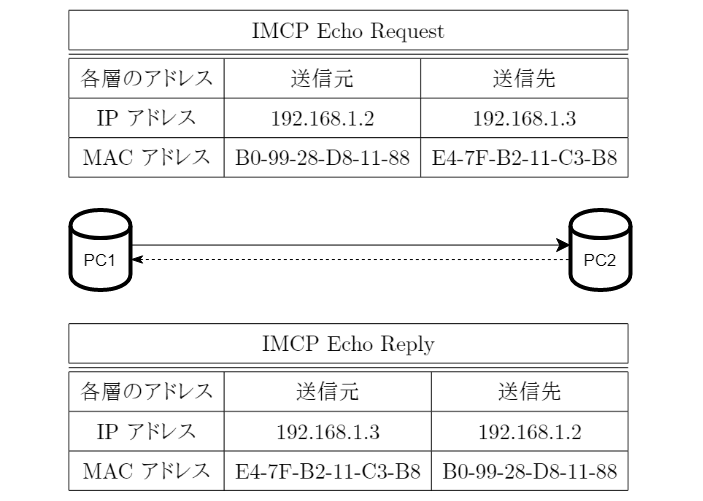
\includegraphics[width=0.7\textwidth]{zu18.png}
		\caption{ICMP のパケット情報}
	\end{figure}
        
    \item キャプチャしたデータの保存
        \begin{itemize}
            \item キャプチャした内容をテキストとしてコピーする。 \\
                (Fileメニュー)から、[Export Packet Dissections]をクリックし、[As Plain Text]をクリックする。ファイル名を指定してテキストファイルとして保存する。このときに画面下部の[Packet Format]の[Packet detail]のチェックをつけて、[All expanded]を指定しておくと詳細な情報を出力できる。
            \item キャプチャしたデータ形式で保存する。\\
                キャプチャしたデータ形式で保存するときはキャプチャソフトを終了する前に情報を保存する。このデータは、後日Wiresharkなどで詳細に分析したい時などに使用できる。 
        \end{itemize}
\end{enumerate}

\section{実験5 ファイアウォールの設定 }

\subsection{実施事項}
\begin{itemize}
    \item パーソナルファイアウォールの設定
    \item 代表的なプロトコルの理解
\end{itemize}
ファイアウォールの基本的なパケットフィルタリングの機能により、不正アクセスを軽減する仕
組みを理解する。ICMP, HTTPの通過制御を行い、pingコマンドやブラウザを使用した通信を遮
断できることを確認する。 

\subsection{使用機器と構成}
2台以上のPCをSwitchで接続し、1台はパーソナルファイアウォール(Windows ファイアウォー
ル)によるアクセス制限を行う。\\
このほかのセキュリティ系ソフトウェアのファイアウォールが動作している場合は、これを一時
的に停止しておくこと。

\subsection{実施手順}
1台のPCにおいて、パーソナルファイアウォールの操作によりパケットの通過を制御する。 
\begin{itemize}
    \item HTTPサーバが起動していることを確認する。
    \item (スタートボタン)を右クリックし、[コントロールパネル]を選択する。[Windows Defender ファ
    イアウォール]を起動する。\\\\ 
        (Windows Defender ファイアウォールの有効化または無効化)をクリックし、図14のように
        有効化していることを確認する。\\\\
        プロトコルや送信元などの詳細な条件を指定して制御する場合は、[Windows Defender ファイ
        アウォール]の[詳細設定]をクリックして、図15の[セキュリティが強化された Windows
        Defender ファイアウォール]のウィンドウ内で指定する。\\\\
        ICMPの遮断とHTTPの遮断を排他的に行い、ファイアウォールで遮断されたPCに対して、他の
        PCからアクセスする。応答時間やエラーメッセージなどのアクセス状況を表10に記入する。 \\
    \item ICMP(pingコマンド)の通信を遮断する。 \\
        受信の規則のICMPv4のエコー要求を受信する制御条件を選択し、右側の操作で[規則の無効化]
        をすることでpingに応じなくなる。結果の確認後に、設定を元に戻す。 
    \item Webサーバ側でHTTPを遮断する。\\
        受信の規則のポート番号TCP/80番を受信する制御条件を選択し、右側の操作で[規則の無効化]
        をすることでHTTPサーバプロセスへのアクセスを遮断する。ブラウザで確認後に、設定を元に戻
        す。 
            \begingroup
            \setlength{\tabcolsep}{5pt} % Default value: 6pt
            \renewcommand{\arraystretch}{1.5} % Default value: 1
                \begin{table}[H]
                \centering
            	\caption{遮断したプロトコルとアクセスの状況}
            	\begin{tabular}{|l|l|l|}
            	    \hline
            	    アクセスの方法 &ICMPの遮断時 & HTTPの遮断時 \\[0.5ex]
            		\hline\hline
                	pingの結果 & 無 & 有 \\ \hline
                    Webアクセスの結果 & 有 & 無 \\ \hline
            	\end{tabular}
                \end{table} 
            \endgroup
            \begin{center}
            \underline{重要:ファイアウォールの設定は必ず元の[有効]、[許可/ブロック]の設定に戻しておくこと。} 
            \end{center}
     オプションで実施: 
     \item ICMPを遮断するときにパケットのキャプチャを行い、どのような動きになっているかを確認
            する。 
      \item ICMPを遮断したときと、存在しないIPアドレスにpingを行ったときの結果は、どちらも通信
            ができない。このときの動作の違いをキャプチャして確認する。このときも、pingの前にARPテー
            ブルのクリアを行うこと。 
\end{itemize}

\section{実験6 IPv6を使用した通信 }

\subsection{実施事項}
\begin{itemize}
    \item  IPv6アドレスによるPC間の疎通確認 
\end{itemize}
    LAN内の通信にIPv6アドレスを使用することで、IPv6アドレスの仕様と設定などの基本的な操
    作方法をIPv4アドレスと比較して理解する。 

\subsection{使用機器類と構成 }

実験2のケーブルと機器の接続と同じ構成で、IPアドレスだけをIPv6に変更する。 

\subsection{実施手順}
LANの物理的接続を行い、PCにIPv6グローバルユニキャストアドレスを設定してPC間の疎通の
確認を行う。 

\begin{enumerate}
    \item IPv6アドレスの設定
        \begin{itemize}
            \item IPv4と同様に、図16の[インターネット プロトコル バージョン6(TCP/IPv6)]を選択し、
                IPv6アドレスを入力する。\\\\
                PCに入力するIPv6アドレス 2001:db8:x::n/64 \\
                自分が割り当てたIPv6アドレス 2001:db8:4::1/64 \\
                \text{*}ここで、xは実験グループごとに割り当てる番号とし、nは1から増加して各PCに付与する。\\\\
                なお、IPv6アドレスについての詳細は、JPNICのWebサイトなどを参照せよ。\\
                \underline{https://www.nic.ad.jp/jp/newsletter/No32/090.html}
            \item ipconfigコマンドを用いて設定されているIPv6アドレスを確認し、表11の情報を記入する。 \\
                1つのインターフェースにIPv6アドレス、一時IPv6アドレス、リンクローカルIPv6アドレスなど
                の複数のアドレスが設定されている。 
        \end{itemize}
                \begingroup
                \setlength{\tabcolsep}{5pt} % Default value: 6pt
                \renewcommand{\arraystretch}{1.5} % Default value: 1
                    \begin{table}[H]
                    \centering
                	\caption{IPv6アドレスの確認結果 }
                	\begin{tabular}{|c|c|c|}
                	    \hline
                	    PC & IPv6アドレス & リンクローカル IPv6 アドレス \\[0.5ex]
                		\hline\hline
                    	PC1 & 2001:db8:1::2 & fe80::c0de:8b8b:d02b:bf08\%5 \\ \hline
                    	PC2 & 2001:db8:1::3 & fe80::d187:43ad:2c29:263\%13 \\ \hline
                    	PC3 & 2001:db8:1::4 & fe80::edb7:230:3966:cc00\%9 \\ \hline
                    	PC4 & 2001:db8:1::5 & fe80::e191:a654:b7dd:71fa \\ \hline
                	\end{tabular}
                    \end{table} 
                \endgroup
    \item IPv6アドレスを使用した通信状況の確認
        \begin{itemize}
            \item pingコマンドを使用して、PC間で通信ができることを確認する。\\\\
                  \textbf{C:>ping -6 2001:db8:4::2} \\
                 2001:db8:4::2にpingを送信しています 32バイトのデータ:\\
                 2001:db8:4::2からの応答:時間 < 1ms \\
           \item また、宛先にリンクローカルIPv6アドレスを指定して、pingコマンドにより同様に通信がで
                    きることを確認する。 
            \item ブラウザで各PCから相手側のPC(Webサーバ)のIPv6アドレスを指定してアクセスし、Webペー
                    ジが表示されることを確認する。
                なお、ブラウザなどにIPv6アドレスを入力するときは、[2001:db8:1::2]のように[]で囲んで入
                力する。
            
        \end{itemize}
\end{enumerate}

\section{検討事項}

\subsection{検討事項1}
\begin{itemize}
    \item WANとLANの概要、利用面でのこれらの関係、および設置者(工事をする者)の違いについて。\\
    \underline{WAN (Wide Area Network)}は 遠く離れた場所とつながったネットワークのこと。WANは簡単に言えばLANとLANをつないだ大きなネットワークである。\\
    \underline{LAN (Local Area Network)}は広くても一施設内程度の規模で用いられるコンピュータネットワークのことである。 \\
    \underline{利用面でのこれらの関係}\\ LANで構築した小規模のコンピュータネットワーク同士を接続する際に、WANが使用される。 例えば、工場に構築したLANを他の工場と接続、企業同士の接続などである。 \\
    \underline{設置者(工事をする者)の違いについて }\\
    WANは地理的に離れた場所を接続する必要があるため、利用者個人が配線をするこ とができず、NTTなどの電気通信業者に設置を依頼する必要がある。またWANの設 置だけではインターネットに接続することはできず、別途プロバイダ業者と契約を行う必要がある。 
    LANは家庭内や企業内など限定された範囲のネットワークのため、一般の人でも構築ができる
\end{itemize}

\subsection{検討事項2}
\begin{itemize}
    \item リピータHUBと比較したSwitchの機能の特徴について \\
        スイッチングハブ(switching hub)は宛先の端末にのみ信号を中継するのに 対し、リピータハブ(repeater hub)は宛先に関係なくつながれている全ての端末に信号を中継する。
        リピータハブは、送信先に関わらず送られてきたパケットをすべてのポートに送信するた め、端末Aから端末Bにデータを送信している間は、ほかの端末同士が通信を行うこ とはできない。一方Switchは、送られてきたデータを、MACアドレスをもとに判別 することで、送信先の端末にだけデータを送信するため、端末Aから端末Bへデータ を送信する場合、データはほかの端末を経由せずに、直接送信先へ届けられる。この ため、無駄なデータ転送が行われず、ネットワーク全体の負荷が軽くなるという特徴 がある。端末Aから端末Bへデータを送ると同時に、端末Cから端末Dへデータを 送るといった、複数同時通信も可能である。 
 
\end{itemize}

\pagebreak

\section{吟味}


\subsection{実験1 LANケーブルの作成}
この実験ではLANケーブルを実際に作成することで、LANケーブル(ツイストペアケーブル)の構造を理解することができた。また、LANケーブルは2本のケーブルを撚り合わせて1ペアとした形状のものを4ペア8芯にしたタイプのツイストペアケーブルが主に使われていることが分かった。そしてLANケーブルはシールドしたSTP(ShieldedTwistedPairCable)と、シールドの無いUTP(UnshieldedTwistedPairCable)の2種類があり、多く使われているのはシールドされていないUTPだということが分かった。

\subsection{実験2 Switchを使用したLANの構築}
この実験では本来PCで自動的に割り振られるIPアドレスを手動で任意のIPアドレスに変更する方法やパソコンの物理アドレス(MAC Address)を確認する方法について理解することできた。

\subsection{実験3 撚りを解いたケーブルでの通信 }
この実験で撚りを解いた3m、5m、10mのケーブルと普通の100mツイストのケーブルで通信状態の確認を行ったところ、100mツイストケーブルでは通信することができたが、撚りを解いた3m、5m、10mのケーブルを使用した場合は通信出来なかった。この結果からツイストペアケーブルは、1対ごとに線を捻ることでクロストークをキャンセルし、本来の信号のみが流れるようになっており、この撚りを解くとクロストークをキャンセルできなくなり、本来の信号以外のノイズが流れてしまって通信できないということが分かった。

\subsection{実験4 パケットのモニタリング}
ARPのrequestフレームとreplyフレームでは、送信元のMACアドレスとIPアドレスが入れ替わっ
ていることがわかった。また、ICMPのrequestフレームとreplyフレームも同様に入れ替わってい
ることから、ARPのテーブルに記憶されているアドレスと通信をしていることがわかった。
そしてLANにつながっている機器が別の機器と通信するためにはIPアドレスだけではなくMACアドレスも必要であり、そのため、ARPデーブルにはLANに繋がっていて、通信したことがある機器のIPアドレスとMACアドレスをテーブルに保存していて、あるIPアドレスを利用している機器のMACアドレスを知りたい時はこのARPテーブルを参照していることが分かった。

\subsection{実験5 ファイアウォールの設定 }
本実験ではアプリケーション層のファイアウォールを有効にすると、HTTPなどは遮断できるが、ICMPは
遮断できないことがわかった。

\subsection{実験6 IPv6の設定方法}
 本実験ではWindowsでIPv6アドレスを手動で任意のアドレスに変更する方法について理解することができた。
 
 \section{参考文献}
 \begin{itemize}
    \item LANとWANって何が違うの?\\
         https://flets-w.com/user/point-otoku/knowledge/other/otherl28.html
    \item Implementing TCP in Rust \\
        https://youtu.be/bzja9fQWzdA
    \item マスタリングTCP/IP 入門編 第5版 \\
        https://www.ohmsha.co.jp/book/9784274068768/
 
 \end{itemize}
 


\end{document}


\iffalse
 \begingroup
    \setlength{\tabcolsep}{5pt} % Default value: 6pt
    \renewcommand{\arraystretch}{1.5} % Default value: 1
    \begin{table}[H]
    \centering
	\begin{tabular}{|c|c|c|}
	    \hline
	   \multicolumn{3}{|c|}{ICMP Echo Request} \\ \hline
		\hline\hline
    	   各層のアドレス & 送信元 & 送信先 \\ \hline
    	   IPアドレス & 192.168.1.2 & 192.168.1.3 \\ \hline
    	   MACアドレス & B0-99-28-D8-11-88 & E4-7F-B2-11-C3-B8 \\ \hline
    
	\end{tabular}
\end{table} 
\endgroup

\vspace{1.5cm}\\

\begingroup
    \setlength{\tabcolsep}{5pt} % Default value: 6pt
    \renewcommand{\arraystretch}{1.5} % Default value: 1
    \begin{table}[H]
    \centering
	\begin{tabular}{|c|c|c|}
	    \hline
	   \multicolumn{3}{|c|}{ICMP Echo Reply} \\ \hline
		\hline\hline
    	   各層のアドレス & 送信元 & 送信先 \\ \hline
    	   IPアドレス & 192.168.1.3 & 192.168.1.2 \\ \hline
    	   MACアドレス & E4-7F-B2-11-C3-B8 &  B0-99-28-D8-11-88\\ \hline
	\end{tabular}
\end{table} 
\endgroup
\if